\documentclass{article}

% Language setting
% Replace `english' with e.g. `spanish' to change the document language
\usepackage[english]{babel}

% Set page size and margins
% Replace `letterpaper' with `a4paper' for UK/EU standard size
\usepackage[letterpaper,top=2cm,bottom=2cm,left=3cm,right=3cm,marginparwidth=1.75cm]{geometry}

% Useful packages
\usepackage{amsmath}
\usepackage{amsthm}
\usepackage{amsfonts}
\usepackage{graphicx}
\usepackage[colorlinks=true, allcolors=blue]{hyperref}
\newtheorem{theorem}{Theorem}[section]
\newtheorem{corollary}{Corollary}[theorem]
\newtheorem{lemma}[theorem]{Lemma}
\newtheorem{definition}{Definition}

\title{Natural Gradient Descent for Neural Networks with Orthogonal Greedy Approximation}
\author{Luowei Yin}

\begin{document}
\maketitle

\section{Natural gradient}

Consider the PINN loss for a Poisson PDE:
\[
    \mathcal{L}(u_\theta)=\frac{1}{2}\|-\Delta u_\theta - f\|^2_{L^2(\Omega)} + \frac{\tau}{2}\|u_\theta-g\|^2_{L^2(\partial\Omega)}.
\]
One may try to obtain analytically $\nabla_u \mathcal{L}(u^k)$ and approximate a step of gradient descent by neural networks. 
%However this is not feasible since the gradient has the form:
%\[
%    \nabla_u\mathcal{L}(u)=\chi_{\Omega}((-\Delta)^*((-\Delta u - f)))+\tau \chi_{\partial\Omega}(u-g).
%\]
However this is not feasible because the gradient does not exist in $L^2(\Omega)$. %Even if for some other problems that the gradient does exist, it often possesses bad regularity and becomes difficult to approximate with small error. Moreover, in the function gradient descent perspective, this gradient reduces the regularity of $u^k$ and the next step will not make sense. 
Updating $u$ by this gradient will make its regularity insufficient for the state PDE to be solved. If one try to project the gradient by smoothing operator (Ritz map, or Hilbertian approach) $H^{-1}\to H^1$, this amounts to solving another PDE.

Another technique to approximate this function gradient is to use the natural gradients, whose main idea is to project the function gradient into the tangent space of the model manifold. 

Define the manifold $\mathcal{M} = \{u_\theta:\theta\in\mathbb{R}^p\}$,  and the generalized tangent space at $\theta$ by $T_{u_\theta}\mathcal{M}:=\text{span}\{\frac{\partial u_\theta}{\partial\theta_i}:i=1\cdots p\}$. For a infinitesimal move of $\theta$, it generates a move of $u_\theta$ along the manifold. 

\begin{definition}
    Consider an infinitesimal step $\frac{d\theta}{dt}=h$ for some $h\in\mathbb{R}^p$. We have 
    \[ 
        \frac{d u_\theta}{dt}=\sum_{i=1}^p \frac{\partial u_\theta}{\partial \theta_i}\frac{d\theta_i}{dt}=\sum_{i=1}^p \frac{\partial u_\theta}{\partial \theta_i}h_i.
        \] 
    This evolving direction of $u_\theta$ is called the push-forward at $u_\theta$ by $h$, denoted by $\#h$.
\end{definition}

The tangent space is a finite dimensional linear space, consisting of all possible push-forward at $u_\theta$. Note that by the definition of tangent space, 
%the the tangent space is defined to be the range of Frechet derivative, 
it is always a subset of the space where $u_\theta$ lies in. The natural gradient aims to find the best approximation of $\nabla_u \mathcal{L}$ in $T_{u_\theta}\mathcal{M}$, which is given by projection:
\[
    \tilde{\nabla_u} \mathcal{L} = \arg\min_{v\in T_{u_\theta}\mathcal{M}}\|v- \nabla_u\mathcal{L}\|_{L^2(\Omega)}^2 = \Pi_{T_{u_\theta}\mathcal{M}}(\nabla_u\mathcal{L}). 
\]

To find the approximated gradient, it suffices to solve the cofficients $h_i$ with respect to some metric. More specifically, taking the canonical $L^2$ inner product as metric, 
\begin{align*}
    h^* &=  \arg\min_{h\in\mathcal{R}^p}\|\sum_{i=1}^p \frac{\partial u_\theta}{\partial \theta_i}h_i - \nabla_u\mathcal{L}\|_{L^2(\Omega)}^2, \\ 
    \#h^*&=\tilde{\nabla_u} \mathcal{L}.
\end{align*}

If the function gradient $\nabla_u \mathcal{L}$ is not explicitly known or behaves badly such that integrals are diffucult to evaluate, one can apply the following workaround. 

%(Not rigorous)Assuming that $T_{u_\theta}\mathcal{M}$ and $\nabla_u\mathcal{L}$ lie in a same Hilbert space that is seperable and uniformly convex. 
Assuming that $T_{u_\theta}\mathcal{M}$ lies in a separable and uniformly convex Hilbert space. 
Then there is an orthogonal split for $\nabla_u \mathcal{L}$:
\[
    \nabla_u \mathcal{L} = \tilde{\nabla_u} \mathcal{L} + \nabla_u \mathcal{L}^{\perp}.
\]
Where $\tilde{\nabla_u} \mathcal{L}$ is the projcetion part and the orthogonal part $\nabla_u \mathcal{L}^{\perp}$ satisfy $(\nabla_u \mathcal{L}^{\perp},\frac{\partial u_\theta}{\partial\theta i})_{L^2(\Omega)}=0$ for each $i=1\cdots p$. Now we can test $\nabla_u\mathcal{L}$ by each basis function $\frac{\partial u_\theta}{\partial\theta j}$, yielding 
\[
    (\nabla_u \mathcal{L},\frac{\partial u_\theta}{\partial\theta j})_{L^2(\Omega)} = (\tilde{\nabla_u} \mathcal{L},\frac{\partial u_\theta}{\partial\theta j})_{L^2(\Omega)} = \sum_{i=1}^p (\frac{\partial u_\theta}{\partial\theta i},\frac{\partial u_\theta}{\partial\theta j})_{L^2(\Omega)}h^*_i.
\]
An obvious benefit of this formulation comes from $(\nabla_u \mathcal{L},\frac{\partial u_\theta}{\partial\theta j})_{L^2(\Omega)}=\frac{\partial \mathcal{L}}{\partial\theta_j}$ by chain rule. If $u_\theta$ is a neural network, this gradient $\frac{\partial \mathcal{L}}{\partial\theta_j}$ can be easily and precisely obtained by auto-differentiation. The burden of evaluating integrals involving $\nabla_u\mathcal{L}$ is transferred to the Gram matrix. For neural networks, $u_\theta$ is usually smooth, hence integrals in Gram matrix are relatively easier to evaluate. Now it suffices to solve $h^*\in\mathbb{R}^p$ such that 
\[
    Mh^*=\nabla_\theta\mathcal{L}.
\]
where $M$ is the Gram matrix. This is the most common formulation of natural gradients. But numerically the Gram matrix usually becomes singuler during evolution. (is accuracy of $h^*$ really important here?).

In natural gradient descent, solving the gradient descent direction is equivalent to finding the best approximation of function gradient in the tangent space of model manifold with respect to a given metric. The Gram matrix becoming singular implies highly correlated tangent vectors. While, this correlation does not imply reduced expressivity. Several problem are raised here: how to characterize the redundancy of tangent vectors, and is it possible to find a subset of tangent vectors that generates nearly best approximation of function gradient? When the training gets stuck at a local minima, it means the function gradient becomes orthogonal to the tangent space. The natural gradient displays another possibility that the tangent vectors are heavily "clustered" and becomes non informative. 

\subsection{Orthogonal Greedy Algorithm}
The Gram matrix becoming singular implies the increasing correlation of tangent vectors, and a degradation of tangent space. When tangent vectors are highly correlated, the projection error onto tangent space becomes large, hence gradient descent becomes less effective. Hence the following method is motivated to reduce the redundancy of tangent vectors by choosing only several, instead of all basis vectors that achieves a good approximation of target gradient.

Selecting $k$ tangent vectors that minimize a projection error of $\nabla_u\mathcal{L}$ is generally infeasible, since it requires to go through all the combinations. We may instead try to do this in a sequential greedy manner. Suppose each gradient descent step only one parameter is to be updated, the optimal choice of tangent vector is trivially given by:
\begin{align}
    i_1&=\arg\min_{i=1\cdots p}\|\nabla_u \mathcal{L}-\frac{(\nabla_u \mathcal{L},\frac{\partial u_\theta}{\partial\theta i})_{L^2(\Omega)}}{\|\frac{\partial u_\theta}{\partial\theta i}\|^2}\frac{\partial u_\theta}{\partial\theta i}\|^2 \\
    &=\arg\max_{i=1\cdots p} \frac{|\partial_{\theta_i}\mathcal{L}|}{\|\frac{\partial u_\theta}{\partial\theta i}\|}
\end{align}

This produces a residual defined as $r_1=\nabla_u\mathcal{L}-\Pi_{H_1}(\nabla_u\mathcal{L})$, where $H_1=\text{span}(\partial_{\theta_{i_1}}u_{\theta})$. Continuing this approach, the second vector best approxiamtes the residual $r_1$:
\begin{align}
    i_2&=\arg\min_{i=1\cdots p}\|r_1-\frac{(r_1,\frac{\partial u_\theta}{\partial\theta i})_{L^2(\Omega)}}{\|\frac{\partial u_\theta}{\partial\theta i}\|^2}\frac{\partial u_\theta}{\partial\theta i}\|^2 
\end{align}

Hence the algorithm is summarized as follows:

Denote: Index set of selected basis $I_k$, linear space spanned by index set $H_k:=\text{span}\{\partial_{\theta_i}u_\theta, i\in I_k\}$. Residual $r_k:=\nabla_u\mathcal{L}-\Pi_{H_k}(\nabla_u\mathcal{L})$, and the coefficient vector $h_k$ of $\Pi_{H_k}(\nabla_u \mathcal{L})$ in the tangent space. The one-dimensional subspace spanned by each $\partial_{\theta_i}u_\theta$ is denoted by $S_i$. Initialize $I_0=\emptyset$, the $(k+1)$-th new index to be added into $I$ is given by:
\begin{align*}
    i_{k+1}&=\arg\min_{i\notin I_k}\|r_k-\Pi_{S_i}(r_k)\|^2 \\ 
    &= \arg\min_{i\notin I_k}\|r_k-\frac{(r_k,\frac{\partial u_\theta}{\partial\theta i})_{L^2(\Omega)}}{\|\frac{\partial u_\theta}{\partial\theta i}\|^2}\frac{\partial u_\theta}{\partial\theta i}\|^2 \\ 
    &= \arg\min_{i\notin I_k} \frac{(r_k,\frac{\partial u_\theta}{\partial\theta i})^2}{\|\frac{\partial u_\theta}{\partial\theta i}\|^2}-2\frac{(r_k,\frac{\partial u_\theta}{\partial\theta i})^2}{\|\frac{\partial u_\theta}{\partial\theta i}\|^2} \\ 
    &= \arg\max_{i\notin I_k} \frac{|(r_k,\frac{\partial u_\theta}{\partial\theta i})|}{\|\frac{\partial u_\theta}{\partial\theta i}\|} 
\end{align*}

Since $r_k=\nabla_u\mathcal{L}-\Pi_{H_k}(\nabla_u\mathcal{L})=\nabla_u\mathcal{L}-(G_{[I_k]}^{-1} (\nabla_\theta\mathcal{L})_{k,[I_k]})^T [\partial_{\theta_i}u_\theta,i\in I_k]$, we have 
\begin{align*}
    i_{k+1}&= \arg\max_{i\notin I_k} \frac{|(r_k,\frac{\partial u_\theta}{\partial\theta i})|}{\|\frac{\partial u_\theta}{\partial\theta i}\|} \\ 
    &=\arg\max_{i\notin I_k} \frac{|(\nabla_u\mathcal{L}-(G_{[I_k]}^{-1} (\nabla_\theta\mathcal{L})_{k,[I_k]})^T [\partial_{\theta_i}u_\theta,i\in I_k],\frac{\partial u_\theta}{\partial\theta i})|}{\|\frac{\partial u_\theta}{\partial\theta i}\|}  \\ 
    &= \arg\max_{i\notin I_k} \frac{|(\nabla_u\mathcal{L},\frac{\partial u_\theta}{\partial\theta i})-((G_{[I_k]}^{-1} (\nabla_\theta\mathcal{L})_{k,[I_k]})^T [\partial_{\theta_i}u_\theta,i\in I_k],\frac{\partial u_\theta}{\partial\theta i})|}{\|\frac{\partial u_\theta}{\partial\theta i}\|} \\ 
    &= \arg\max_{i\notin I_k} \frac{|\partial_{\theta_i}\mathcal{L}-((G_{[I_k]}^{-1} (\nabla_\theta \mathcal{L})_{k,[I_k]})^T [\partial_{\theta_i}u_\theta,i\in I_k],\frac{\partial u_\theta}{\partial\theta i})|}{\|\frac{\partial u_\theta}{\partial\theta i}\|} \\ 
    &= \arg\max_{i\notin I_k} \frac{|\partial_{\theta_i}\mathcal{L}-(Gh_k)_{[i]}|}{\|\frac{\partial u_\theta}{\partial\theta i}\|} \\ 
    &= \arg\max_{i\notin I_k} \frac{|\nabla_{\theta}\mathcal{L}-Gh_k|}{[\|\frac{\partial u_\theta}{\partial\theta i}\|,i=1\cdots p]}.
\end{align*}
where the division in last line is element-wise. Note that all matrix and vectors are pre-computed, hence no integration is needed during iteration. Once a new index is obtained, we update:
\[
    I_{k+1}=I_{k}\cap\{i_{k+1}\}, h_{k+1,[I_{k+1}]}=G^{-1}_{[I_{k+1}]}\nabla_\theta\mathcal{L}_{[I_{k+1}]}, h_{k+1,[I_{k+1}^c]}=0.
\]
Iterating over $k=1\cdots K$, we obtain a sequence of projection that converges to the best approximation of $\nabla_u\mathcal{L}$ in the tangent space. Moreover, the residual is also non-increasing in norm, ans can be estimated by:
\begin{align*}
    \|r_k\|^2 = (Gh_k-2\nabla_\theta\mathcal{L})^T h_k + C
\end{align*}
where the constant $C=\|\nabla_u\mathcal{L}\|^2$ is fixed during iteration.

\section{Numerical evidence}
\subsection{Testing on least squares}
We test the performance of NGD on least squares problem:
\[
    \min_{\theta\in\mathbb{R}^p} \frac{1}{2}\|u_\theta-g\|^2_{L^2(\Omega)}.
\]
where the data $g=\sin(\pi x)\sin(\pi y )+\sin(\frac{3}{2}\pi x)\sin(\frac{3}{2}\pi y)$, domain $\Omega=[0,1]^2$, and the integral is evaluated by Monte Carlo.

\subsubsection*{Test on shallow networks}
Layers: $[2,30,1]$ with tanh activation function. Target function:
\[
    g = \sin(\pi x)\sin(\pi y )+\sin(\frac{3}{2}\pi x)\sin(\frac{3}{2}\pi y)
\]
Logarithmic grid search in interval $[0,1]$ with 30 grids. Greedy step is 10. Parameter gradient will not be cut. Preconditioned gradient is the 
minimum-norm solution.

\begin{figure}[hbt]
    \centering
    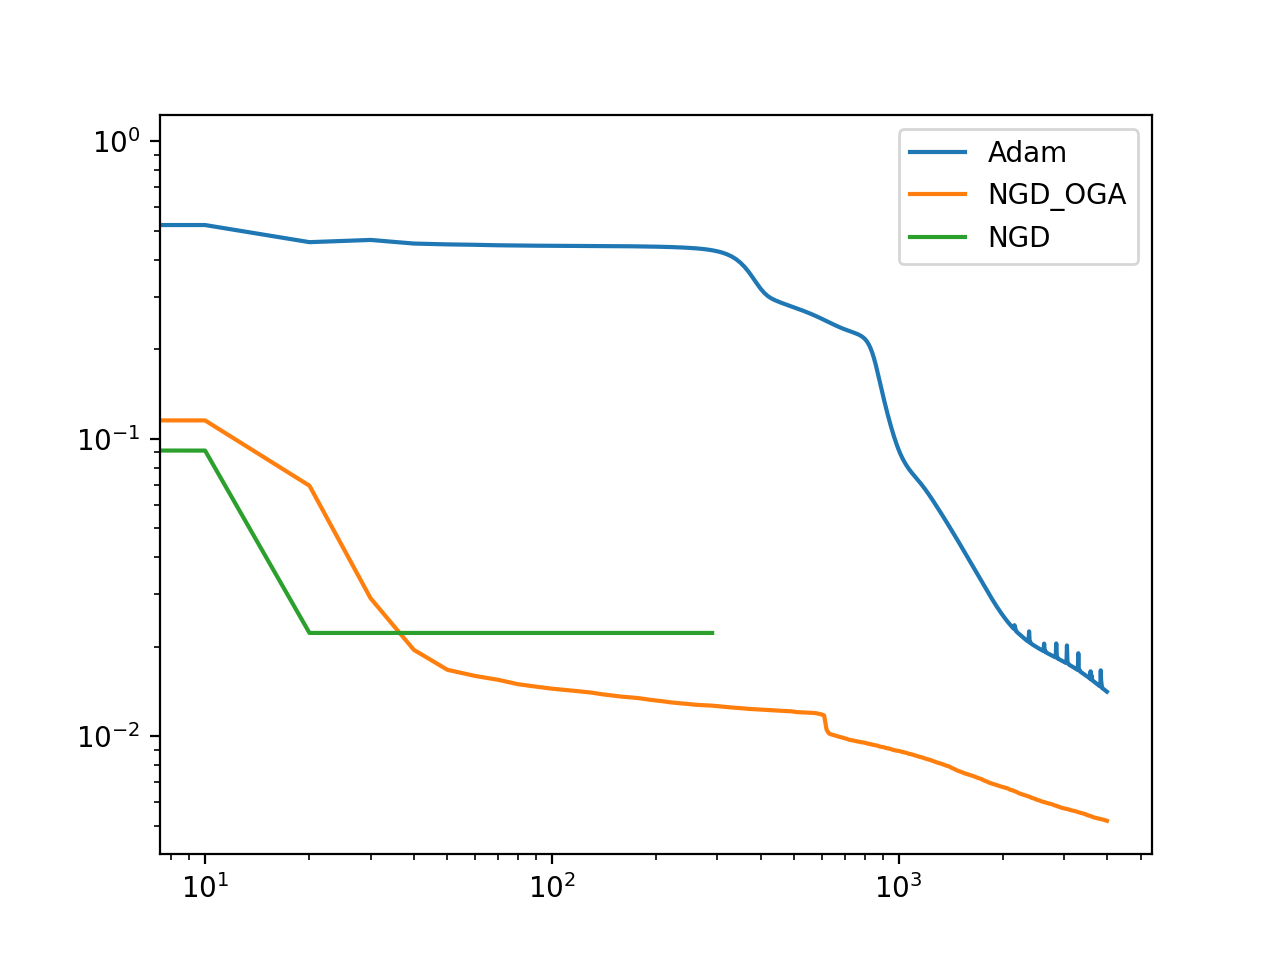
\includegraphics[width=0.6\textwidth]{figures/ls_plot.png}
\label{fig:lsplot}
\caption{Least sqaures by shallow NN.}
\end{figure}

\subsubsection*{Test on multilayer perceptron}
Layers: $[2,20,20,1]$ with tanh activation. Greedy step is 20. Parameter gradient will not be cut. Preconditioned gradient is the minimum-norm solution. 

\begin{figure}[hbt]
    \centering
    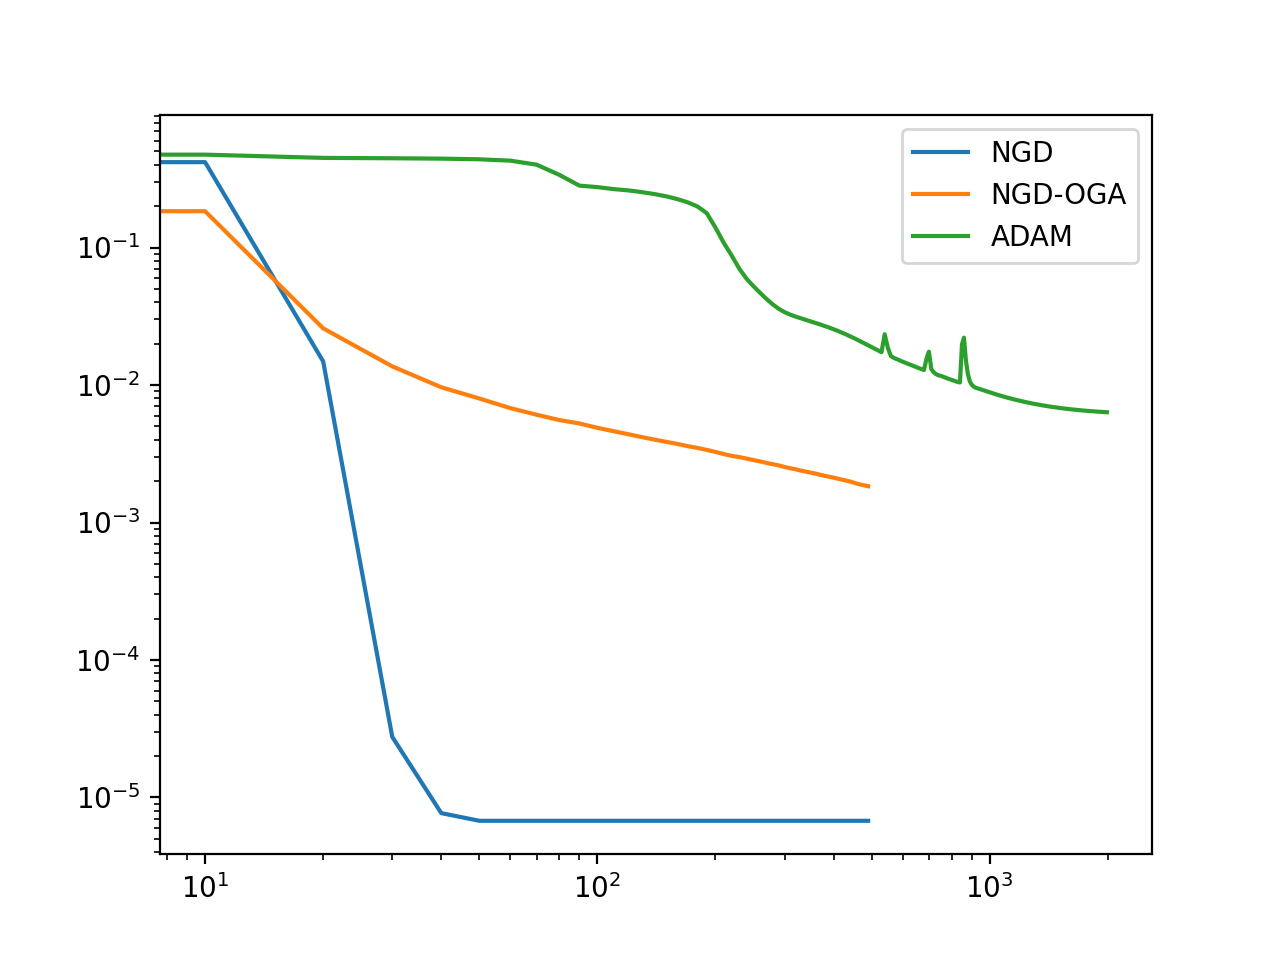
\includegraphics[width=0.6\textwidth]{figures/ls_mlp.png}
\label{fig:lsplot2}
\caption{Least sqaures by multilayer NN.}
\end{figure}

%\subsubsection*{Will the greedy algorithm slow down the convergence?}
%In the greedy algorithm, only a subset of parameter will be updated. Hence a possible issue is the convergence slowering down compared with standard NGD. In this case, one has to integrate the Gram matrix more times, which in turn increases the computational cost. 

\subsection{Testing on Poisson PDE}
We test the performance of NGD on 2D Poisson PDE on squared domain, with ground truth $u^*=\sin(\pi x)\sin(\pi y)$. As reported on their paper, the E-NGD sometimes get stuck in local optima and the loss value remains large. There are two possible reasons: 1. in the very first few steps, due to insuitable initialization, the Gram matrix tend to be singular and it yields an astronomically large gradient scale. One can remedy by cutting gradient into a reasonable range, or pre-training by stanrdard gradient descent for a few steps, as commented on paper. 2. Sometimes the Gram matrix is always too singular and in each step the gradient is always large in scale. Cutting gradient does not give a valid descent direction, and not cutting gradient leads to a bad step. Using backtracking line search instead of grid search might help. 

\subsubsection*{Test on Poisson example via E-NGD}
Firstly we compare E-NGD and E-NGD-OGA. The boundary penalty weight is 100, and architecture is layer $[2,20,20,1]$ with tanh activation. To prevent exploding parameter, we cut each parameter gradient into $[-1000,1000]$. Logarithmic grid search is applied to find suitable stepsize. 
\begin{figure}[hbt]
    \centering
    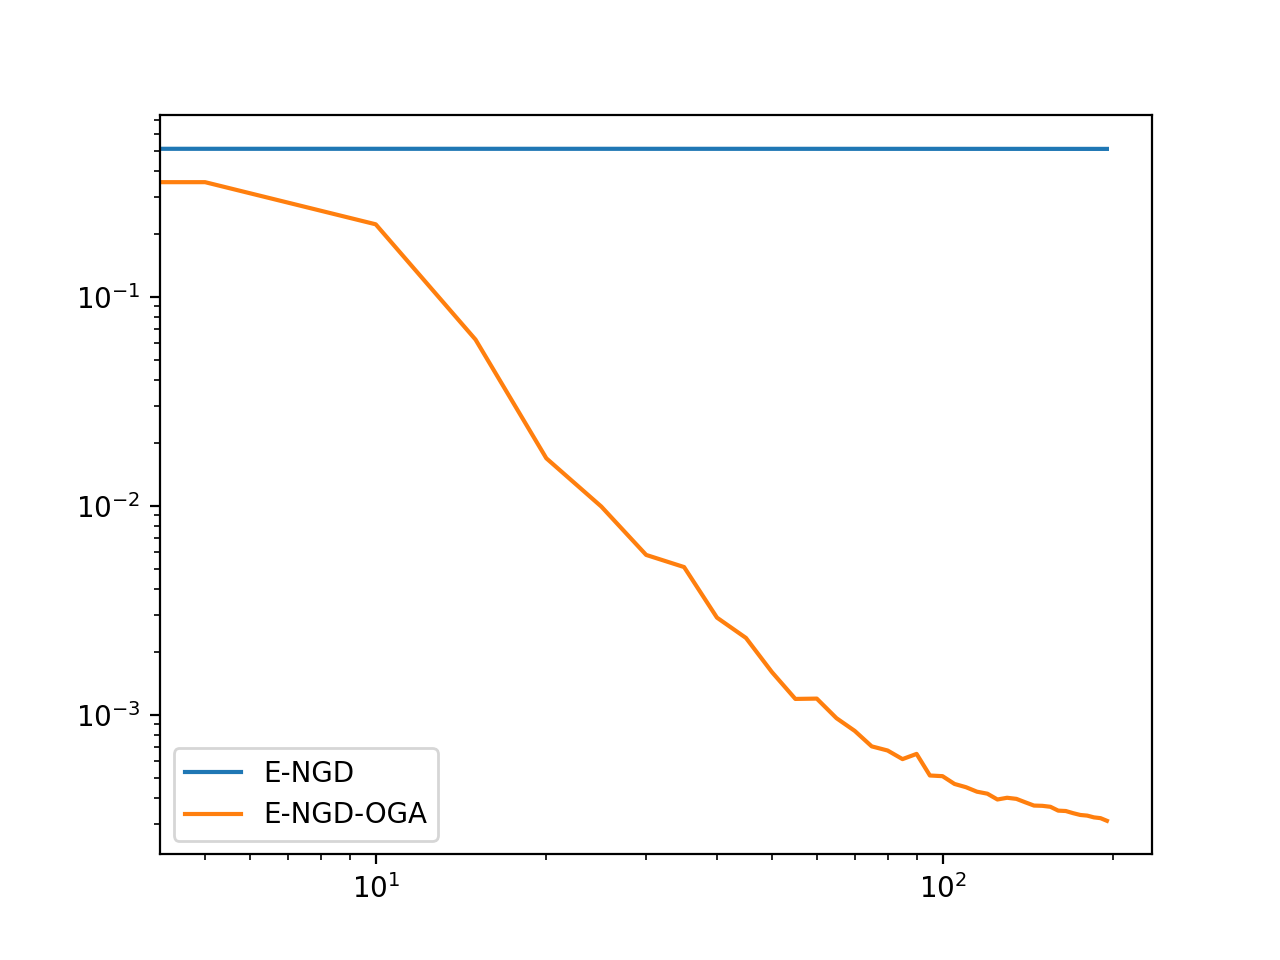
\includegraphics[width=0.6\textwidth]{figures/poissont1.png}
\label{fig:poissont1}
\caption{Poisson test 1.}
\end{figure}



%\bibliographystyle{alpha}
%\bibliography{ref}

\end{document}

\end{document}